\documentclass[10pt,a4paper]{article}
\usepackage[utf8]{inputenc}
\usepackage[parfill]{parskip}
\usepackage[section]{placeins}
\usepackage{subfig}
\usepackage{graphicx}
\usepackage{array}
\usepackage{tabularx}
\usepackage[scientific-notation=true]{siunitx}
\usepackage{amsmath}
\usepackage{hyperref}

\author{Dominik Nerger (i6146759)}
\title{Text Mining South Park}
\date{\today}

\begin{document}
	\maketitle
	
	\tableofcontents
	
	\section{Introduction}
	
	
	The repository is available on GitHub\footnote{\url{https://github.com/dnerger/South-Park-Text-Mining}}.
	
	\section{Data set}	
	The data set spans from seasons \textbf{1} to \textbf{18}, adding up to 257 episodes overall with a file size of 5.41MB. It contains 70896 rows, with each row possessing information about the \textbf{season}, \textbf{episode}, \textbf{character} and \textbf{line}. 
	
	The data set has been crawled by Bob Adams and is available to download on GitHub\footnote{\url{https://github.com/BobAdamsEE/SouthParkData}}. It has been assembled by crawling the South Park Archives\footnote{\url{http://southpark.wikia.com/wiki/South_Park_Archives}}. 
	
	The code of GitHub repository is not available to the public. An attempt at a crawl is available in the GitHub repository.
	
	
	\begin{figure}[h]
	\centering
	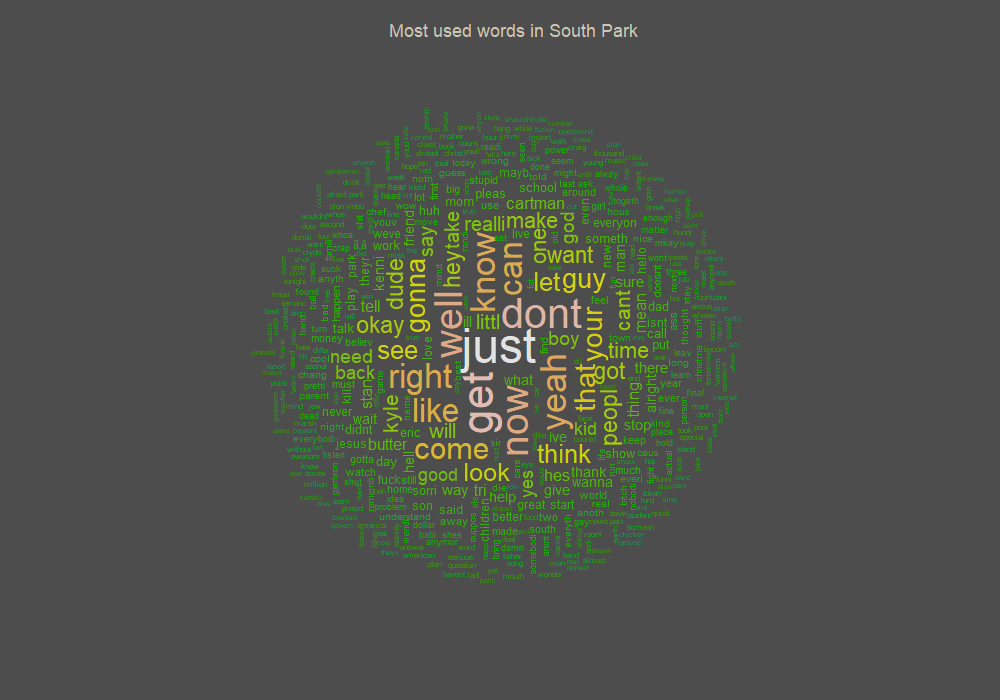
\includegraphics[scale=0.9]{images/WordCloud.png}
	\caption{General wordcloud, containing terms by frequency}
	\label{fig:WordCloud}
	\end{figure}
	
	\begin{figure}[h]
	\centering
	\includegraphics[scale=0.9]{images/WordCloud-TFIDF.png}
	\caption{General wordcloud, containing terms by TF-IDF score}
	\label{fig:WordCloud-TFIDF}
	\end{figure}
	\begin{figure}[h]
	\centering
	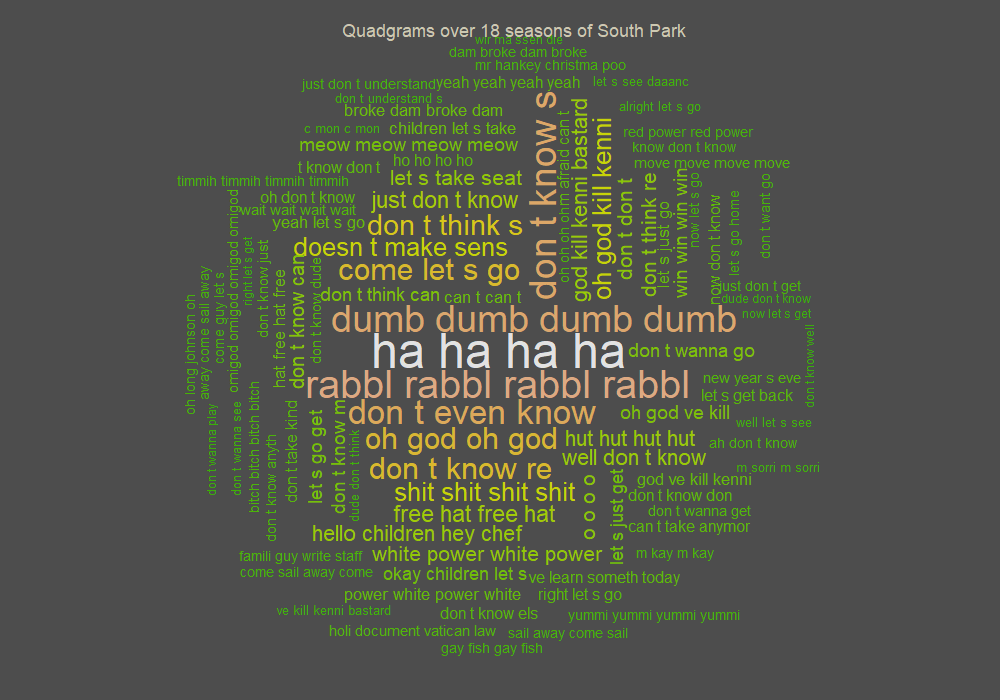
\includegraphics[scale=0.9]{images/WordCloud-ngram.png}
	\caption{Wordcloud containing ngrams (n=4) by frequency}
	\label{fig:WordCloud-ngram}
	\end{figure}
	
	\begin{figure}[h]
	\centering
	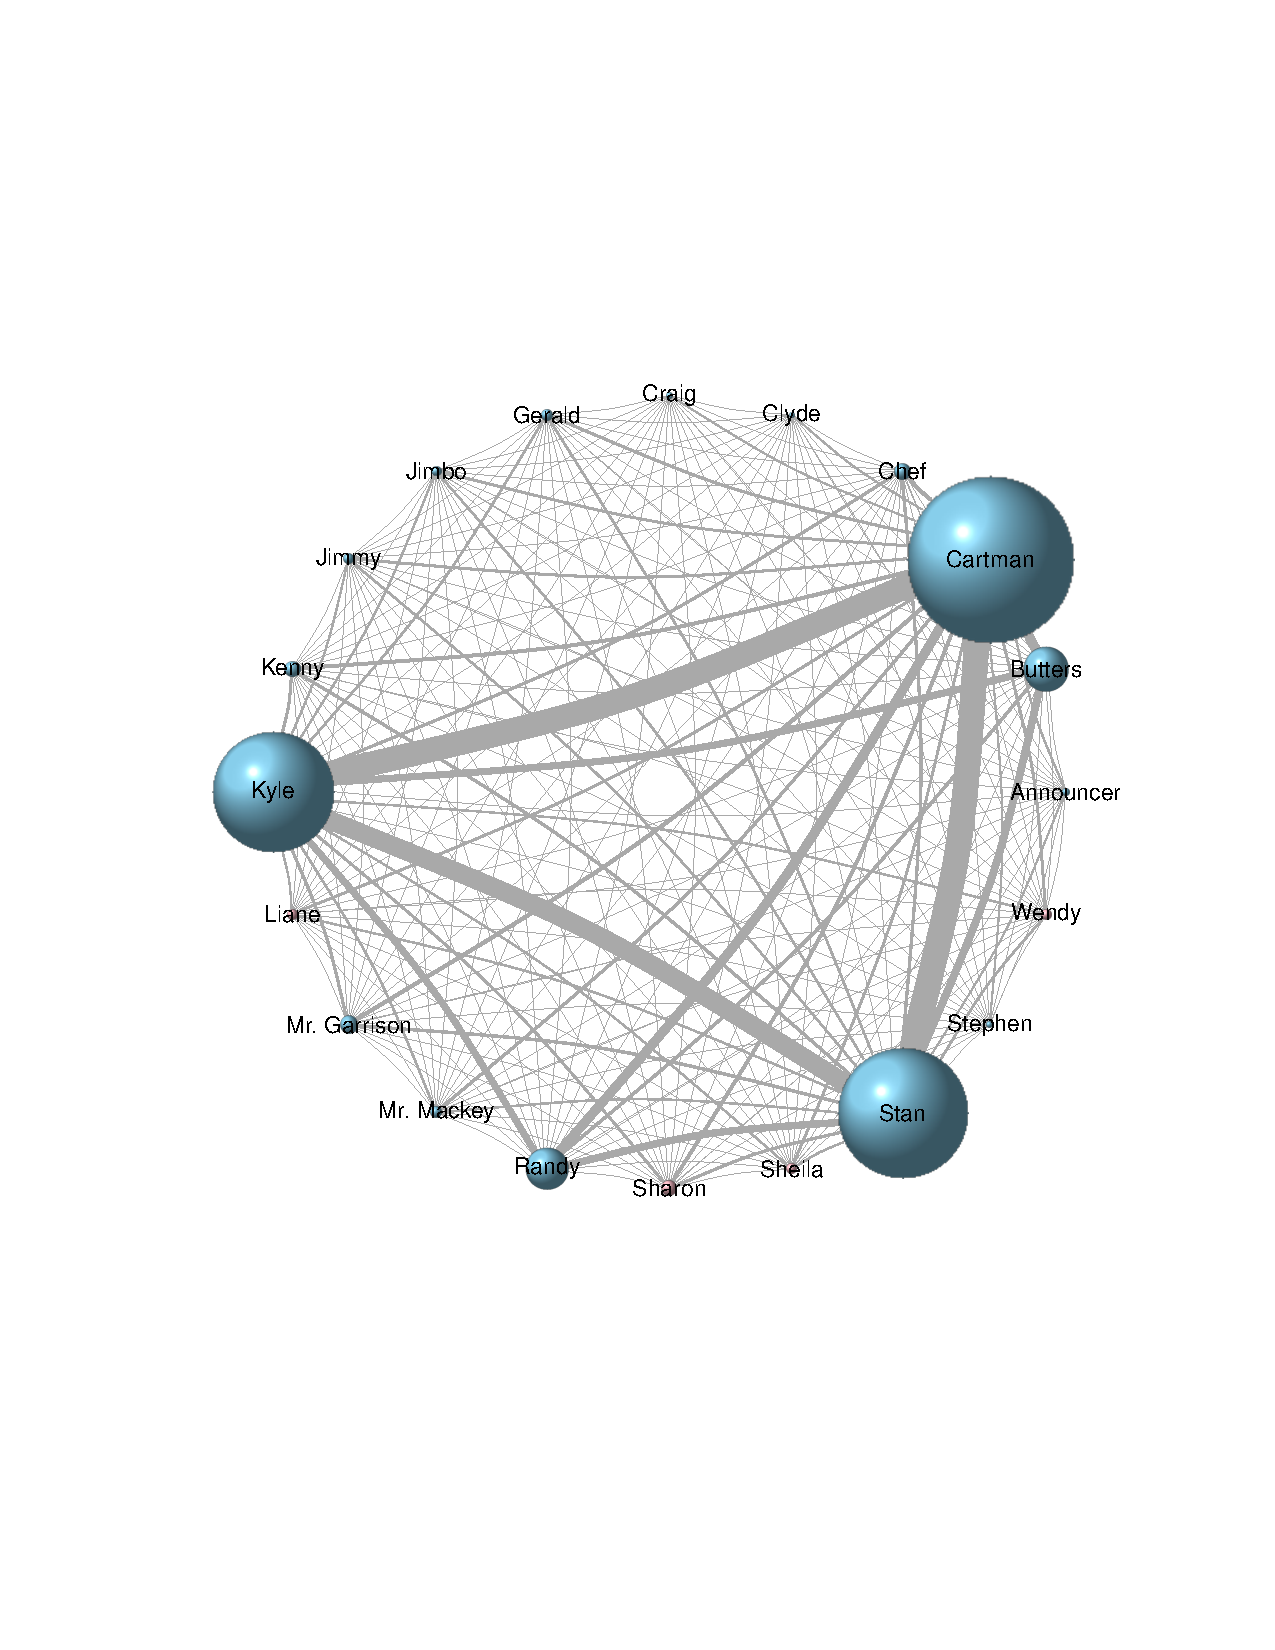
\includegraphics[scale=0.7]{images/CoOccurence Matrix.pdf}
	\caption{Co-occurences of characters over 257 episodes, size of vertex in relation to amount of lines}
	\label{fig:CoOccurence}
	\end{figure}
	
	\section{Libraries}
	
	All scripts have been programmed in \textit{R}. To execute the scripts, R needs to be installed. To view temporary files that are executed during runtime, e.g. the corpus or a TermDocumentMatrix, it is advised to install RStudio. The libraries necessary for each script are imported at the top of each script, if they are not installed they can be installed by executing:
	
	\begin{verbatim}
	install.packages("library-name")
	\end{verbatim}
	
	In the following, all libraries that are related to Text Mining techniques will be introduced.
	
	The library \textbf{tm} is the Text Mining package of R, which enables pre-processing of data sets and allows to build the corpus. \textbf{RWeka} is a collection of machine learning algorithms for data mining tasks. \textbf{NMF} introduces the Non-negative Matrix Factorization to R.
	\textbf{NLP} and \textbf{OpenNLP} are libraries that provide Natural Language Processing techniques and are used for NER-Tagging. \textbf{syuzhet} extracts sentiments from text and contains the three sentiment dictionaries \textit{bing}, \textit{afinn} and \textit{nrc}.
	The package \textbf{stm} is used for Structural Topic Modeling  which is LDA with additional met-data and can be visualized using the package \textbf{LDAvis}.
	Libraries used for visualization include \textbf{igraph},\textbf{ggplot2}, \textbf{ggraph}, \textbf{viridis} and \textbf{wordcloud}.
	
	\section{Pre-processing}
	
	
	\section{Implementation and results}
	
	
	\section{Conclusion}
	In conclusion, 

	\section{Future work}
\end{document}
